% License: LaTeX Project Public License 1.3c
% file aimc2026.tex
% This is the LaTeX source for the instructions to authors using
% the LaTeX2e document class 'aimc2026.cls' for contributions to
% the Conference on AI Music Creativity.

% if you need to pass options to natbib, use, e.g.:
%     \PassOptionsToPackage{numbers, compress}{natbib}
% before loading aimc2026

\documentclass{aimc2026}

\usepackage[utf8]{inputenc} % allow utf-8 input
\usepackage[T1]{fontenc}    % use 8-bit T1 fonts
\usepackage{hyperref}       % hyperlinks
\hypersetup{
  colorlinks = true,  % Colours links instead of ugly boxes
  urlcolor   = blue,  % Colour for external hyperlinks
  linkcolor  = black, % Colour of internal links
  citecolor  = black  % Colour of citations
}
\usepackage{url}            % simple URL typesetting
\usepackage{booktabs}       % professional-quality tables
\usepackage{amsfonts}       % blackboard math symbols
\usepackage{nicefrac}       % compact symbols for 1/2, etc.
\usepackage{microtype}      % microtypography
\usepackage{graphicx}       % figures
\usepackage{cleveref}       % automatic figure references


\hyphenation{% Add custom hyphenations here, separated by space or newline
  hy-phe-na-tion
}

\title{\LaTeX{} Template for the Conference on AI Music Creativity (AIMC) 2026}

% The \author macro works with any number of authors. There are two commands
% used to separate the names and addresses of multiple authors: \And and \AND.
%
% Using \And between authors leaves it to LaTeX to determine where to break the
% lines. Using \AND forces a line break at that point. So, if LaTeX puts 3 of 4
% authors names on the first line, and the last on the second line, try using
% \AND instead of \And before the third author name.

\author{%
  First Author\thanks{Use footnote for providing further information
    about author (webpage, alternative address)---\emph{not} for acknowledging
    funding agencies.} \\
  Department of Music\\
  Strawberry-Raspberry University\\
  Pittsburgh, PA 15213 \\
  \texttt{rhino@music.strawberry-raspberry.edu} \\
  % examples of more authors
  \And
  Coauthor \\
  Affiliation \\
  Address line 1 \\
  Address line 2 \\
  \texttt{email} \\
  % \AND
  % Coauthor \\
  % Affiliation \\
  % Address \\
  % \texttt{email} \\
  % \And
  % Coauthor \\
  % Affiliation \\
  % Address \\
  % \texttt{email} \\
  % \And
  % Coauthor \\
  % Affiliation \\
  % Address \\
  % \texttt{email} \\
}

\begin{document}


\twocolumn[%
  \maketitle
  \begin{abstract}
    The abstract paragraph should be indented 1.5~cm on both the left- and right-hand margins.
    Use 10~point type, with a vertical spacing (leading) of 11~points.
    The word \textbf{Abstract} must be centered, bold, and in point size 12. Two line spaces precede the abstract. The abstract
    must be limited to one paragraph.
  \end{abstract}%
]

\aimcnotice % name of proceedings title in the first column bottom

\section{Submission of papers to AIMC 2026}
\label{sec:submissions}

AIMC requires electronic submissions. You can access the submission site via this year's conference website:  \url{https://aimc2026.org/}.

Please read the instructions below carefully and follow them precisely.

When submitting, please omit all author details.


\section{General formatting instructions}
\label{sec:general_instructions}

The page must be DIN A4 size with 2~cm margins on all sides.
The column separation is 8~mm. Use 10-point
type with 11-point vertical spacing (leading). Times New Roman is the
preferred typeface and will be selected by default.
Paragraphs should be separated by \nicefrac{1}{2}~line space (5.5 points), with no
indentation.

The paper title should be 17-point, in initial caps/lower case, bold, centered.
All pages should start at 2~cm from the
top of the page.

In the final version, the authors' names should be in bold, with each name centered above the corresponding address. The lead author's name should be listed first (leftmost), followed by the co-authors' names (if the addresses are different). If there is only one co-author, list the author and co-author side by side.

Please pay special attention to the instructions in \Cref{sec:others}
regarding figures, tables, acknowledgments, and references.

\section{Headings: first level}
\label{sec:headings}

All headings should be flush left.
First-level headings should be written in all caps, bold and in 10-point type.

\subsection{Headings: second level}
\label{sec:headings_second}

Second-level headings should be bold and in 10-point type.

\subsubsection{Headings: third level}
\label{sec:headings_third}

Third-level headings should be in 10-point type.


\section{Citations, figures, tables, references}
\label{sec:others}

\subsection{Citations within the text}
\label{sec:citations}

The \texttt{natbib} package will be loaded for you by default.
Citations must  be author/year.

The documentation for \texttt{natbib}+ may be found at
\begin{center}
  \url{http://mirrors.ctan.org/macros/latex/contrib/natbib/natnotes.pdf}
\end{center}

Instead of using the command "\texttt{\textbackslash cite}," use "\texttt{\textbackslash citep}" for your citations. This will produce citations in round brackets, such as "\citep{partiexample,bookexample}.
If you want to include the author's name in your text, use the command cite, which produces citations appropriate for use in inline text.

For example,
\begin{verbatim}
   \citet{confexample} investigated\dots
\end{verbatim}
produces
\begin{quote}
 \citet{confexample} investigated\dots
\end{quote}

% If you wish to load the \texttt{natbib} package with options, you may add the
% following before loading the \texttt{aimc2026} package:
% \begin{verbatim}
%    \PassOptionsToPackage{options}{natbib}
% \end{verbatim}

Since the submission process is double-blind, refer to your own published work in the third person. That is, use ``In the previous work of Jones et al.\ (Jones et al., 2020),'' not ``In our previous work (Jones et al., 2020).'' If you cite your other papers that are not widely available (e.g., a journal paper under review), use anonymous author names in the citation, e.g., an author of the form ``A.\ Anonymous.''

\subsection{Figures}
\label{sec:figures}

\begin{figure*}[ht]
  \centering
  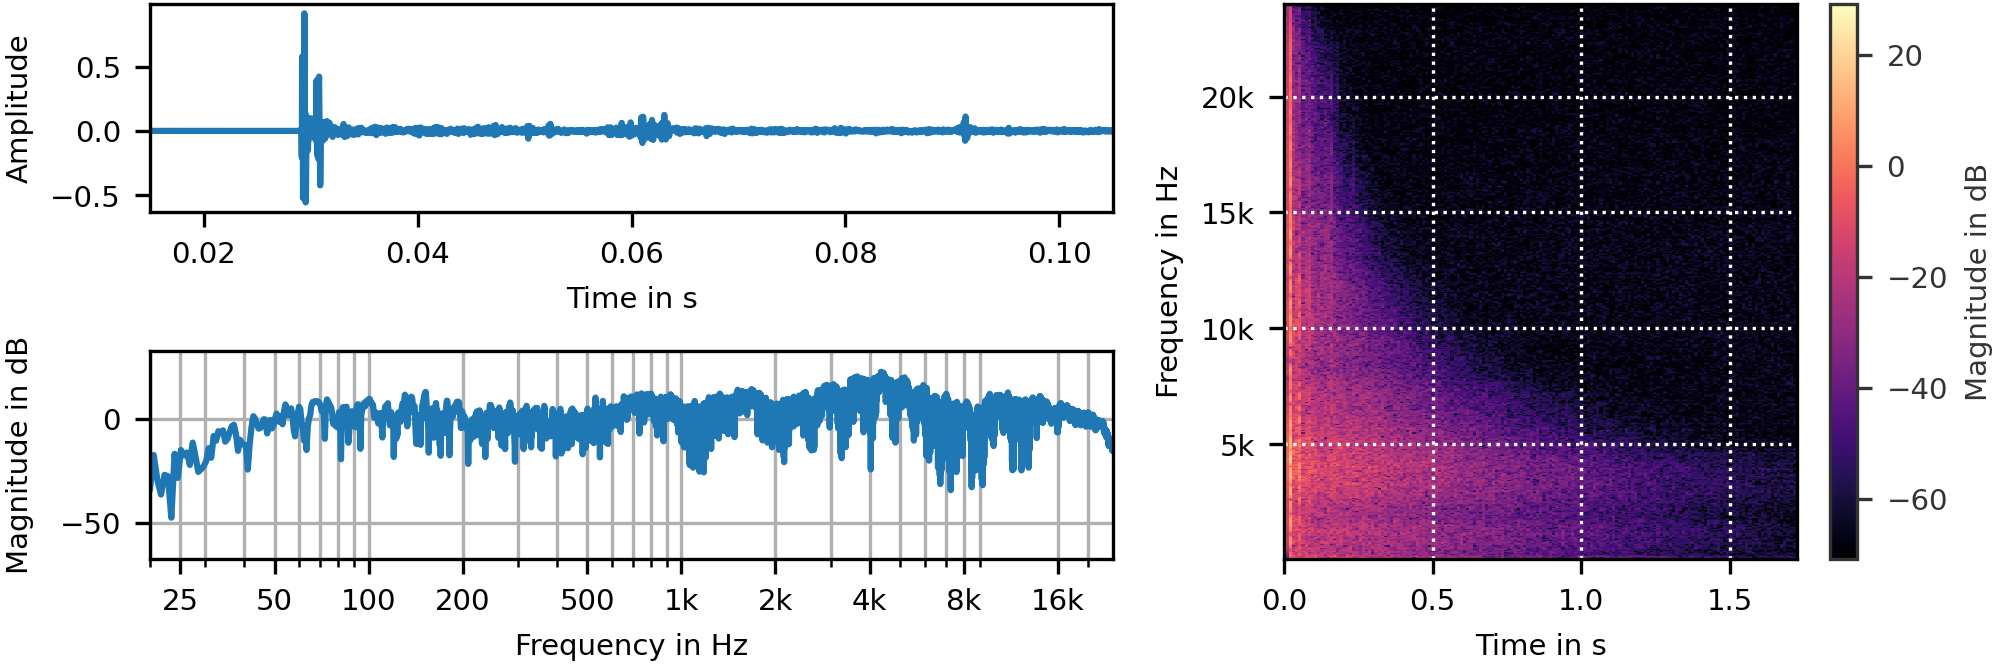
\includegraphics[width=\linewidth]{images/double_column_figure}
  \caption{
    Two-column figures can be placed using the \texttt{figure*} environment.
    The width of the two columns is 17~cm (6.69~in).
  }
  \label{fig:double_column}
\end{figure*}

\begin{figure}[ht]
  \centering
  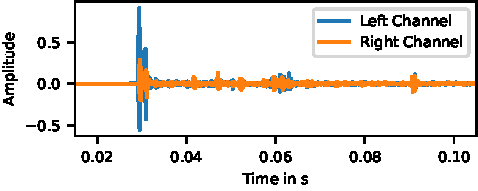
\includegraphics[width=\linewidth]{images/single_column_figure.pdf}
  \caption{
    Single column figures can be placed with the \texttt{figure} environment.
    The text width of a single column is 8.1~cm (3.19~in).
  }
  \label{fig:single_column}
\end{figure}

All artwork must be neat, clean, and legible. Lines should be dark enough for purposes of reproduction. The figure number and caption always appear after the figure. Place one line space before the figure caption and one line space after the figure. Figure captions should be in lowercase, except for the first word and proper nouns. Figures are numbered consecutively.

You may use color figures.  However, it is best for the figure captions and the paper body to be legible if the paper is printed in either black andwhite or color.

Most of the margin problems come from figures positioned by hand using
\texttt{\textbackslash special} or other commands.
We suggest using the command \texttt{\textbackslash includegraphics} from the \texttt{graphicx} package.
Always specify the width as a multiple of the line width:
\begin{verbatim}
  \includegraphics
    [width=1.0\linewidth]{myfile.pdf}
\end{verbatim}
See Section 4.4 in the graphics bundle documentation
\url{http://mirrors.ctan.org/macros/latex/required/graphics/grfguide.pdf}


\subsection{Tables}
\label{sec:tables}

All tables must be centered, neat, clean and legible.  The table number and title always appear before the table.  See \Cref{tab:sample-table}.

Place one line space before the table title and after both the
title and after the table. The table title must be lowercase, except for the first word and proper nouns. Tables are
numbered consecutively.

Note that publication-quality tables \emph{do not contain vertical rules.} We strongly suggest using the \texttt{booktabs} package, which allows you to typeset high-quality, professional tables:
\url{https://www.ctan.org/pkg/booktabs}
This package was used to typeset Table~\ref{tab:sample-table}.

\begin{table}[hbt!]
  \caption{Sample table}
  \label{tab:sample-table}
  \centering
  \begin{tabular}{lll}
    \toprule
    \multicolumn{2}{c}{Part}                   \\
    \cmidrule(r){1-2}
    Name     & Description     & Size in $\mathrm{\mu m}$ \\
    \midrule
    Dendrite & Input terminal  & $\sim$100     \\
    Axon     & Output terminal & $\sim$10      \\
    Soma     & Cell body       & up to $10^6$  \\
    \bottomrule
  \end{tabular}
\end{table}

\subsection{Hyphenation}
\label{sec:hyphenation}

A number of width issues arise when \LaTeX{} cannot properly hyphenate a line. Please give LaTeX hyphenation hints using the \texttt{\textbackslash -} command when necessary.
You can also define custom hyphenations in the preamble using the \texttt{\textbackslash hyphenation} command.
See line 34 of \texttt{aimc2026.tex}.

\subsection{Internal references}
\label{sec:references}

The \texttt{cleveref} package is included in the template.
We suggest using the commands \texttt{cref} and \texttt{Cref} to automatically format references to sections, tables and figures.

Example:

\cref{fig:double_column}, \cref{sec:figures}, \cref{tab:sample-table}. \\
\Cref{fig:double_column}, \Cref{sec:figures}, \Cref{tab:sample-table}.


\subsection{Footnotes}
\label{sec:footnotes}

Footnotes should be used sparingly.  If you do require a footnote, indicate
footnotes with a number\footnote{Sample of the first footnote.} in the
text. Place the footnotes at the bottom of the page on which they appear.
Precede the footnote with a horizontal rule of 2~inches (12~picas).

Note that footnotes are properly typeset \emph{after} punctuation
marks.\footnote{As in this example.}

\section{Final instructions}
\label{sec:final_instructions}

Do not modify any formatting parameters in the style files.  In
particular, do not modify the width or length of the rectangle into which the text should fit, nor the font sizes (except perhaps in the \textbf{References} section; see below). Please note that pages should be numbered.

\section{Preparing PDF files}
\label{sec:pdf_files}

Please prepare your submission files with ``A4'' paper size.

Fonts have been the main cause of problems in the past years. Your PDF file must only contain Type 1 or Embedded TrueType fonts. Here are a few instructions to achieve this.

\begin{enumerate}
  \item You should directly generate PDF files using \texttt{pdflatex}.
  \item You can check which fonts a PDF files uses.  In Acrobat Reader, select the
    menu Files$>$Document Properties$>$Fonts and select Show All Fonts. You can
    also use the program \texttt{pdffonts} which comes with \texttt{xpdf} and is
    available out-of-the-box on most Linux machines.
  \item The IEEE has recommendations for generating PDF files whose fonts are also
    acceptable for AIMC. Please see
    \url{http://www.emfield.org/icuwb2010/downloads/IEEE-PDF-SpecV32.pdf}

  \item \texttt{xfig} "patterned" shapes are implemented with bitmap fonts.  Use
    "solid" shapes instead.
  \item The \texttt{\textbackslash bbold} package almost always uses bitmap fonts.  You should use
    the equivalent AMS Fonts, which is included in this template:
\begin{verbatim}
  \usepackage{amsfonts}
\end{verbatim}
    followed by, e.g., \texttt{\textbackslash mathbb\{R\}}, \texttt{\textbackslash mathbb\{N\}}, or \texttt{\textbackslash mathbb\{C\}}
    for $\mathbb{R}$, $\mathbb{N}$ or $\mathbb{C}$.
    Note that \texttt{amsfonts} is automatically loaded by the \texttt{amssymb} package.
\end{enumerate}

If your file contains type 3 fonts or non embedded TrueType fonts, we will ask
you to fix it.


\section*{Author Declarations}

Author declarations should include conflicts of interest, ethical issues, and comments on the use of AI.

Use unnumbered first level headings for the acknowledgments.
All acknowledgments go at the end of the paper before the list of references.

Do {\bf not} include acknowledgments in the anonymized submission, only in the final paper. You can use the \texttt{ack} environment provided in the style file to automatically hide this section in the anonymized submission.

% \section*{References}

\bibliographystyle{apalike}
\bibliography{references}

References follow the author declarations. Use unnumbered first-level heading for the references. Citation style should follow APA. It is permissible to reduce the font size to \texttt{small} (9 point) when listing the references.

\end{document}